\section{THỰC NGHIỆM VÀ ĐÁNH GIÁ HIỆU NĂNG}

Chương này trình bày các minh chứng thực tế khi chạy mô hình trên giao diện Mininet CLI nhằm khẳng định toàn bộ lý thuyết thiết kế ở Chương 2 đều hoạt động thành công.

\subsection{Kiểm tra trạng thái Hội tụ Định tuyến (OSPF Convergence)}
Bước đầu tiên là xác nhận các Router lõi (P, PE) của ISP đã tìm thấy nhau và hoàn thành việc trao đổi bảng định tuyến. 
Lệnh kiểm tra: \texttt{pe1 vtysh --vty\_socket /tmp/frr\_pe1 -c "show ip ospf neighbor"}

\begin{figure}[H]
    \centering
    % [NOTE] TRONG TERMINAL, SAU KHI CHẠY MAIN_TOPOLOGY.PY, HÃY GÕ LỆNH TRÊN, CHỤP ẢNH MÀN HÌNH CHỨA KẾT QUẢ HIỂN THỊ CỘT STATE LÀ "Full/-" RỒI LƯU VÀO FOLDER image/ TÊN LÀ ospf_neighbor.png
    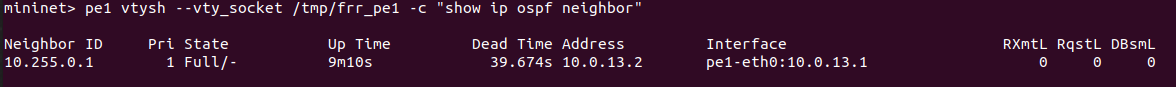
\includegraphics[width=0.8\textwidth]{image/ospf_neighbor.png}
    \caption{Trạng thái láng giềng OSPF đạt trạng thái hội tụ Full}
    \label{fig:ospf_nei}
\end{figure}

\textit{\textbf{Giải thích minh chứng:}} Hình \ref{fig:ospf_nei} cho thấy giao thức OSPF đã thiết lập láng giềng thành công. Dựa vào kết quả trả về, ta thấy Router PE1 đã nhận diện được Neighbor ID là \texttt{10.255.0.1} (địa chỉ Loopback của Router P1) thông qua cổng giao tiếp \texttt{pe1-eth0} có IP \texttt{10.0.13.1}. Trạng thái (State) đạt mức \textbf{Full/-} với thời gian duy trì liên tục (Up Time) là \textbf{9m10s}. Trạng thái \texttt{Full} chứng minh thuật toán Dijkstra đã chạy xong, cơ sở dữ liệu LSDB đã được đồng bộ hóa hoàn toàn giữa Router biên PE1 và Router lõi mạng P1, đảm bảo không có vòng lặp định tuyến.

\subsection{Minh chứng cơ chế cấp phát Nhãn MPLS (LDP Label Distribution)}
Định tuyến mới chỉ cung cấp đường đi. Để tốc độ được đẩy lên cực đại, LDP phải cấp nhãn thành công. 
Ta truy xuất bảng định tuyến chi tiết trên một Router lõi bất kỳ (Router P1) bằng lệnh: \texttt{p1 vtysh --vty\_socket /tmp/frr\_p1 -c "show ip route"}

\begin{figure}[H]
    \centering
    % [NOTE] GÕ LỆNH TRÊN TRONG TERMINAL. CHỤP MÀN HÌNH BẢNG ĐỊNH TUYẾN CÓ CÁC DÒNG CHỮ "label 24", "label 25" VÀ LƯU THÀNH mpls_forwarding.png TRONG FOLDER image/
    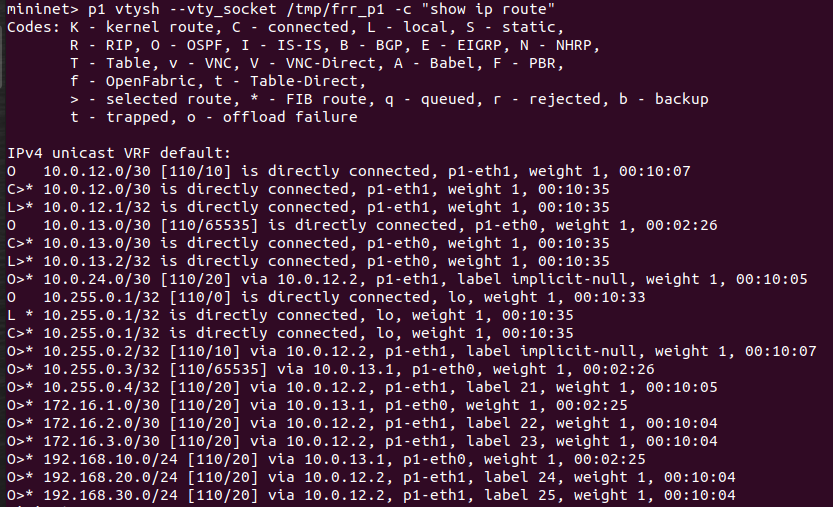
\includegraphics[width=0.8\textwidth]{image/mpls_forwarding.png}
    \caption{Bảng định tuyến xuất hiện Nhãn MPLS (Label) trên Router Core P1}
    \label{fig:mpls_table}
\end{figure}

\textit{\textbf{Giải thích minh chứng:}} Các đường mạng có ký hiệu \texttt{O>*} ở đầu dòng mang ý nghĩa là các tuyến đường ưu tiên nhất được học qua giao thức OSPF. Đáng chú ý nhất, trong Hình \ref{fig:mpls_table}, Router lõi P1 đã học được chính xác dải mạng LAN riêng tư của khách hàng: \texttt{192.168.10.0/24}, \texttt{192.168.20.0/24} và \texttt{192.168.30.0/24} với Up Time hơn \textbf{9-10 phút}. Điều này khẳng định cơ chế Redistribute Static ở PE đã bơm thành công thông tin vào mạng lõi.
Quan trọng hơn cả, ở các tuyến đường trỏ về mạng LAN của khách hàng thông qua cổng trung chuyển \texttt{p1-eth1} (như \texttt{192.168.20.0} và \texttt{192.168.30.0}), ta có thể thấy rõ sự xuất hiện của tham số \textbf{label 24} và \textbf{label 25}. Đối với tuyến đường về \texttt{192.168.10.0/24}, router hiển thị \textbf{label implicit-null} (cơ chế PHP gỡ nhãn sớm). Đây là minh chứng rõ ràng nhất, mang tính quyết định để khẳng định LDP đã chạy và cấp nhãn thành công cho các mạng IP. Gói tin khi đi qua mạng lõi sẽ được gán nhãn này để hoán đổi với tốc độ cao ở lớp 2.5 mà không cần tra cứu IP.

\subsection{Đánh giá thông mạch Ping và tính ẩn danh cấu trúc mạng lõi (Traceroute)}
Khi toàn bộ OSPF và MPLS đã hoàn thành, ta đứng từ một máy tính của nhân viên ở Chi nhánh A (Mạng Flat) và gửi yêu cầu Ping sang một máy ở Chi nhánh B (Mạng 3 lớp).
Lệnh chạy: \texttt{hA1 ping -c 4 192.168.20.11}

\begin{figure}[H]
    \centering
    % [NOTE] GÕ LỆNH TRÊN. CHỤP MÀN HÌNH TRẢ VỀ REPLY TỪ 192.168.20.11 BÁO LOSS = 0% VÀ LƯU THÀNH ping_success.png
    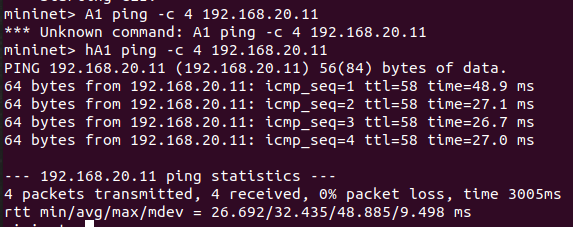
\includegraphics[width=0.8\textwidth]{image/ping_success.png}
    \caption{Kiểm tra thông mạch Ping xuyên chi nhánh thành công}
    \label{fig:ping_test}
\end{figure}

Cuối cùng là việc dùng Traceroute để phân tích đường đi gói tin qua môi trường ISP:
Lệnh: \texttt{hA1 traceroute -n 192.168.30.11}

\begin{figure}[H]
    \centering
    % [NOTE] GÕ LỆNH TRÊN. CHỤP ẢNH MÀN HÌNH TRACEROUTE (TRONG ĐÓ CÓ NHỮNG DÒNG * * * Ở BƯỚC NHẢY SỐ 3 VÀ SỐ 4). LƯU ẢNH THÀNH traceroute_mpls.png
    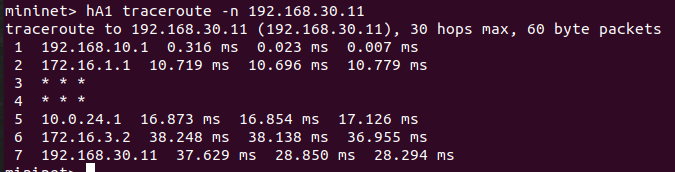
\includegraphics[width=0.8\textwidth]{image/traceroute_mpls.png}
    \caption{Traceroute chứng minh tính ẩn danh và bảo mật của cấu trúc mạng lõi ISP}
    \label{fig:traceroute}
\end{figure}

\textit{\textbf{Giải thích minh chứng:}} Traceroute trong Hình \ref{fig:traceroute} vạch ra con đường mà gói tin đã đi. Tại hop thứ 3 và thứ 4 (nơi gói tin thực sự đang di chuyển trong các Router P của MPLS Backbone), kết quả trả về là \textbf{* * *}. Đây không phải là lỗi rớt mạng (vì Ping vẫn thành công 0\% Loss), mà là đặc trưng bảo mật cực kỳ ưu việt của mạng MPLS (cơ chế ẩn IP lõi hay Disable TTL-Propagation). Router lõi chỉ đọc "Nhãn Lớp 2.5" và không phản hồi gói tin ICMP Lớp 3, giúp nhà cung cấp dịch vụ ISP giấu hoàn toàn cấu trúc liên kết mạng lõi của họ khỏi người dùng cuối, chống lại các cuộc tấn công dò quét mạng diện rộng.
